\documentclass[conference, a4paper]{IEEEtran}

\usepackage{cite}
\usepackage{amsmath,amssymb,amsfonts}
\usepackage{algorithmic}
\usepackage{graphicx}
\usepackage{textcomp}
\usepackage{xcolor}
\usepackage{hyperref}
\usepackage{listings}

\lstset{
    basicstyle=\ttfamily\footnotesize,
    breaklines=true,
    captionpos=b,
    frame=single,
    tabsize=2,
    language=VHDL,
    keywordstyle=\color{blue},
    commentstyle=\color{green!60!black},
    stringstyle=\color{red}
}

\def\BibTeX{{\rm B\kern-.05em{\sc i\kern-.025em b}\kern-.08em
    T\kern-.1667em\lower.7ex\hbox{E}\kern-.125emX}}

\begin{document}

\title{Comprehensive Analysis of Side-Channel Vulnerabilities in RSA Hardware: A Methodological Study on CPA and SPA}

\author{\IEEEauthorblockN{Orhun Boydak}
\IEEEauthorblockA{\textit{Cryptography and Hardware Security Research} \\
Ankara, Turkey \\
}}

\maketitle

\begin{abstract}
As cryptographic algorithms become mathematically unbreakable, attackers increasingly target the physical implementations of these algorithms via Side-Channel Analysis (SCA). This paper presents a complete, end-to-end framework for simulating, extracting, and analyzing power leakages in hardware implementations of the RSA algorithm. We explore the bit-serial Montgomery Multiplication architecture and demonstrate how logical state changes manifest as power consumption. A custom VCD (Value Change Dump) parsing pipeline is developed to model the Hamming Distance (HD) of internal registers. Using this pipeline, two primary attacks are executed on 16-bit and 32-bit RSA architectures. First, Correlation Power Analysis (CPA) using the Pearson Correlation Coefficient is applied, successfully cracking the 16-bit key with 50 traces while failing on the 32-bit key due to algorithmic noise. Second, a Simple Power Analysis (SPA) and Timing Attack is conducted, exploiting the unprotected Square-and-Multiply logic to achieve 100\% key recovery from a single trace. Finally, countermeasures against such architectural vulnerabilities are discussed.
\end{abstract}

\begin{IEEEkeywords}
Side-Channel Analysis (SCA), RSA, Correlation Power Analysis (CPA), Simple Power Analysis (SPA), Hamming Distance, VHDL, Montgomery Multiplication.
\end{IEEEkeywords}

\section{Introduction}
Modern cryptography relies heavily on the computational infeasibility of mathematical problems, such as integer factorization for RSA (Rivest-Shamir-Adleman). However, mathematical robustness does not guarantee the security of the physical device executing the algorithm. When a hardware circuit operates, it consumes power and emits electromagnetic radiation proportional to the data it processes. **Side-Channel Analysis (SCA)** is a domain of hardware security that exploits these unintended physical leakages to extract secret cryptographic keys.

The objective of this research is to construct an end-to-end side-channel simulation environment without the need for expensive physical oscilloscopes. By utilizing Register-Transfer Level (RTL) simulations and parsing the resulting signal transitions, we can mathematically model power consumption and perform academic-grade attacks. 

This paper is structured to define the essential terminology in Section II, detail the hardware architecture in Section III, explain the leakage modeling in Section IV, present the statistical Correlation Power Analysis (CPA) in Section V, and demonstrate a deterministic Simple Power Analysis (SPA) in Section VI.

\section{Theoretical Background and Terminology}
To fully comprehend the attack vectors presented in this paper, several core cryptographic and hardware terminologies must be defined.

\subsection{Side-Channel Analysis (SCA) Fundamentals}
SCA attacks bypass the mathematical strength of an algorithm by observing the physical characteristics of the device. There are two main categories discussed in this study:
\begin{itemize}
    \item \textbf{Simple Power Analysis (SPA):} A technique that involves direct visual or algorithmic observation of a device's power consumption over time. SPA relies on macroscopic pattern differences, such as distinguishing a multiplication operation from an addition operation.
    \item \textbf{Correlation Power Analysis (CPA):} A sophisticated statistical attack. Instead of looking for visual patterns, CPA predicts the power consumption of the device for every possible sub-key guess and uses Pearson Correlation to find the statistical match between the predictions and the actual physical measurements.
\end{itemize}

\subsection{RSA and Square-and-Multiply}
RSA relies on modular exponentiation: $C = M^K \pmod N$. Computing this directly for large numbers is impossible. Hardware implementations utilize the **Square-and-Multiply** algorithm, which processes the binary representation of the key bit-by-bit:
\begin{lstlisting}[language=C]
result = 1;
for (int i = bits-1; i >= 0; i--) {
    result = (result * result) % N; // SQUARE
    if (key[i] == 1) {
        result = (result * M) % N; // MULTIPLY
    }
}
\end{lstlisting}
This algorithm forms the basis of our attacks, as the execution path directly depends on the secret key bit $k_i$.

\subsection{Power Modeling: Hamming Distance (HD)}
In CMOS logic, static power consumption is negligible; power is consumed primarily when logic gates transition from $0 \rightarrow 1$ or $1 \rightarrow 0$. Thus, the power consumed by a register updating its value is proportional to the number of bits that flip. This is called the \textbf{Hamming Distance (HD)}:
\begin{equation}
HD(V_0, V_1) = HW(V_0 \oplus V_1)
\end{equation}
where $HW$ is the Hamming Weight (number of '1's in a binary string).

\subsection{Algorithmic Noise and LFSR}
In an SCA context, any power consumption that does not depend on the specific target register being attacked is considered **Noise**. As the data width of the processor increases (e.g., from 16-bit to 32-bit), the number of gates switching simultaneously increases, drowning out the leakage of a single bit. This is known as **Algorithmic Noise**. To simulate hardware randomness and systemic noise, a Linear Feedback Shift Register (LFSR) is often injected into the hardware environment.

\section{Hardware Architecture and Simulation Pipeline}

The target hardware is a parameterized VHDL implementation of the RSA algorithm, utilizing a bit-serial Montgomery Multiplier to perform modulo arithmetic without division.

\subsection{VHDL Design Structure}
The system is divided into two primary components:
\begin{enumerate}
    \item \texttt{mon\_pro.vhd}: The core Montgomery multiplier that computes $A \times B \times R^{-1} \pmod N$ using bit-serial shifts and additions.
    \item \texttt{mod\_exp.vhd}: The finite state machine (FSM) that orchestrates the Square-and-Multiply loop, repeatedly calling the Montgomery multiplier.
\end{enumerate}

To simulate a realistic target, a 3-bit LFSR (for the 16-bit architecture) and a 32-bit LFSR (for the 32-bit architecture) were synthesized alongside the RSA core to inject dynamic switching noise during operation.

\subsection{The VCD Extraction Engine}
Physical power traces are typically gathered using oscilloscopes. In this pure-software methodology, GHDL is used to generate Value Change Dump (VCD) files containing every logical transition of the circuit. 
A custom Python parsing engine was developed to stream the massive VCD files, track hierarchical scopes (e.g., \texttt{tb\_rsa\_sca.uut\_rsa.mod\_exp\_inst.r\_result}), and calculate the Hamming Distance of the target register precisely at the clock edge.

\section{Power Leakage Modeling}
Before executing an attack, the leakage model must be verified. A single encryption operation was simulated, and the Python parser extracted the dynamic Hamming Distance of the Montgomery Multiplier's internal result register (\texttt{r\_result}).

\begin{figure}[htbp]
\centerline{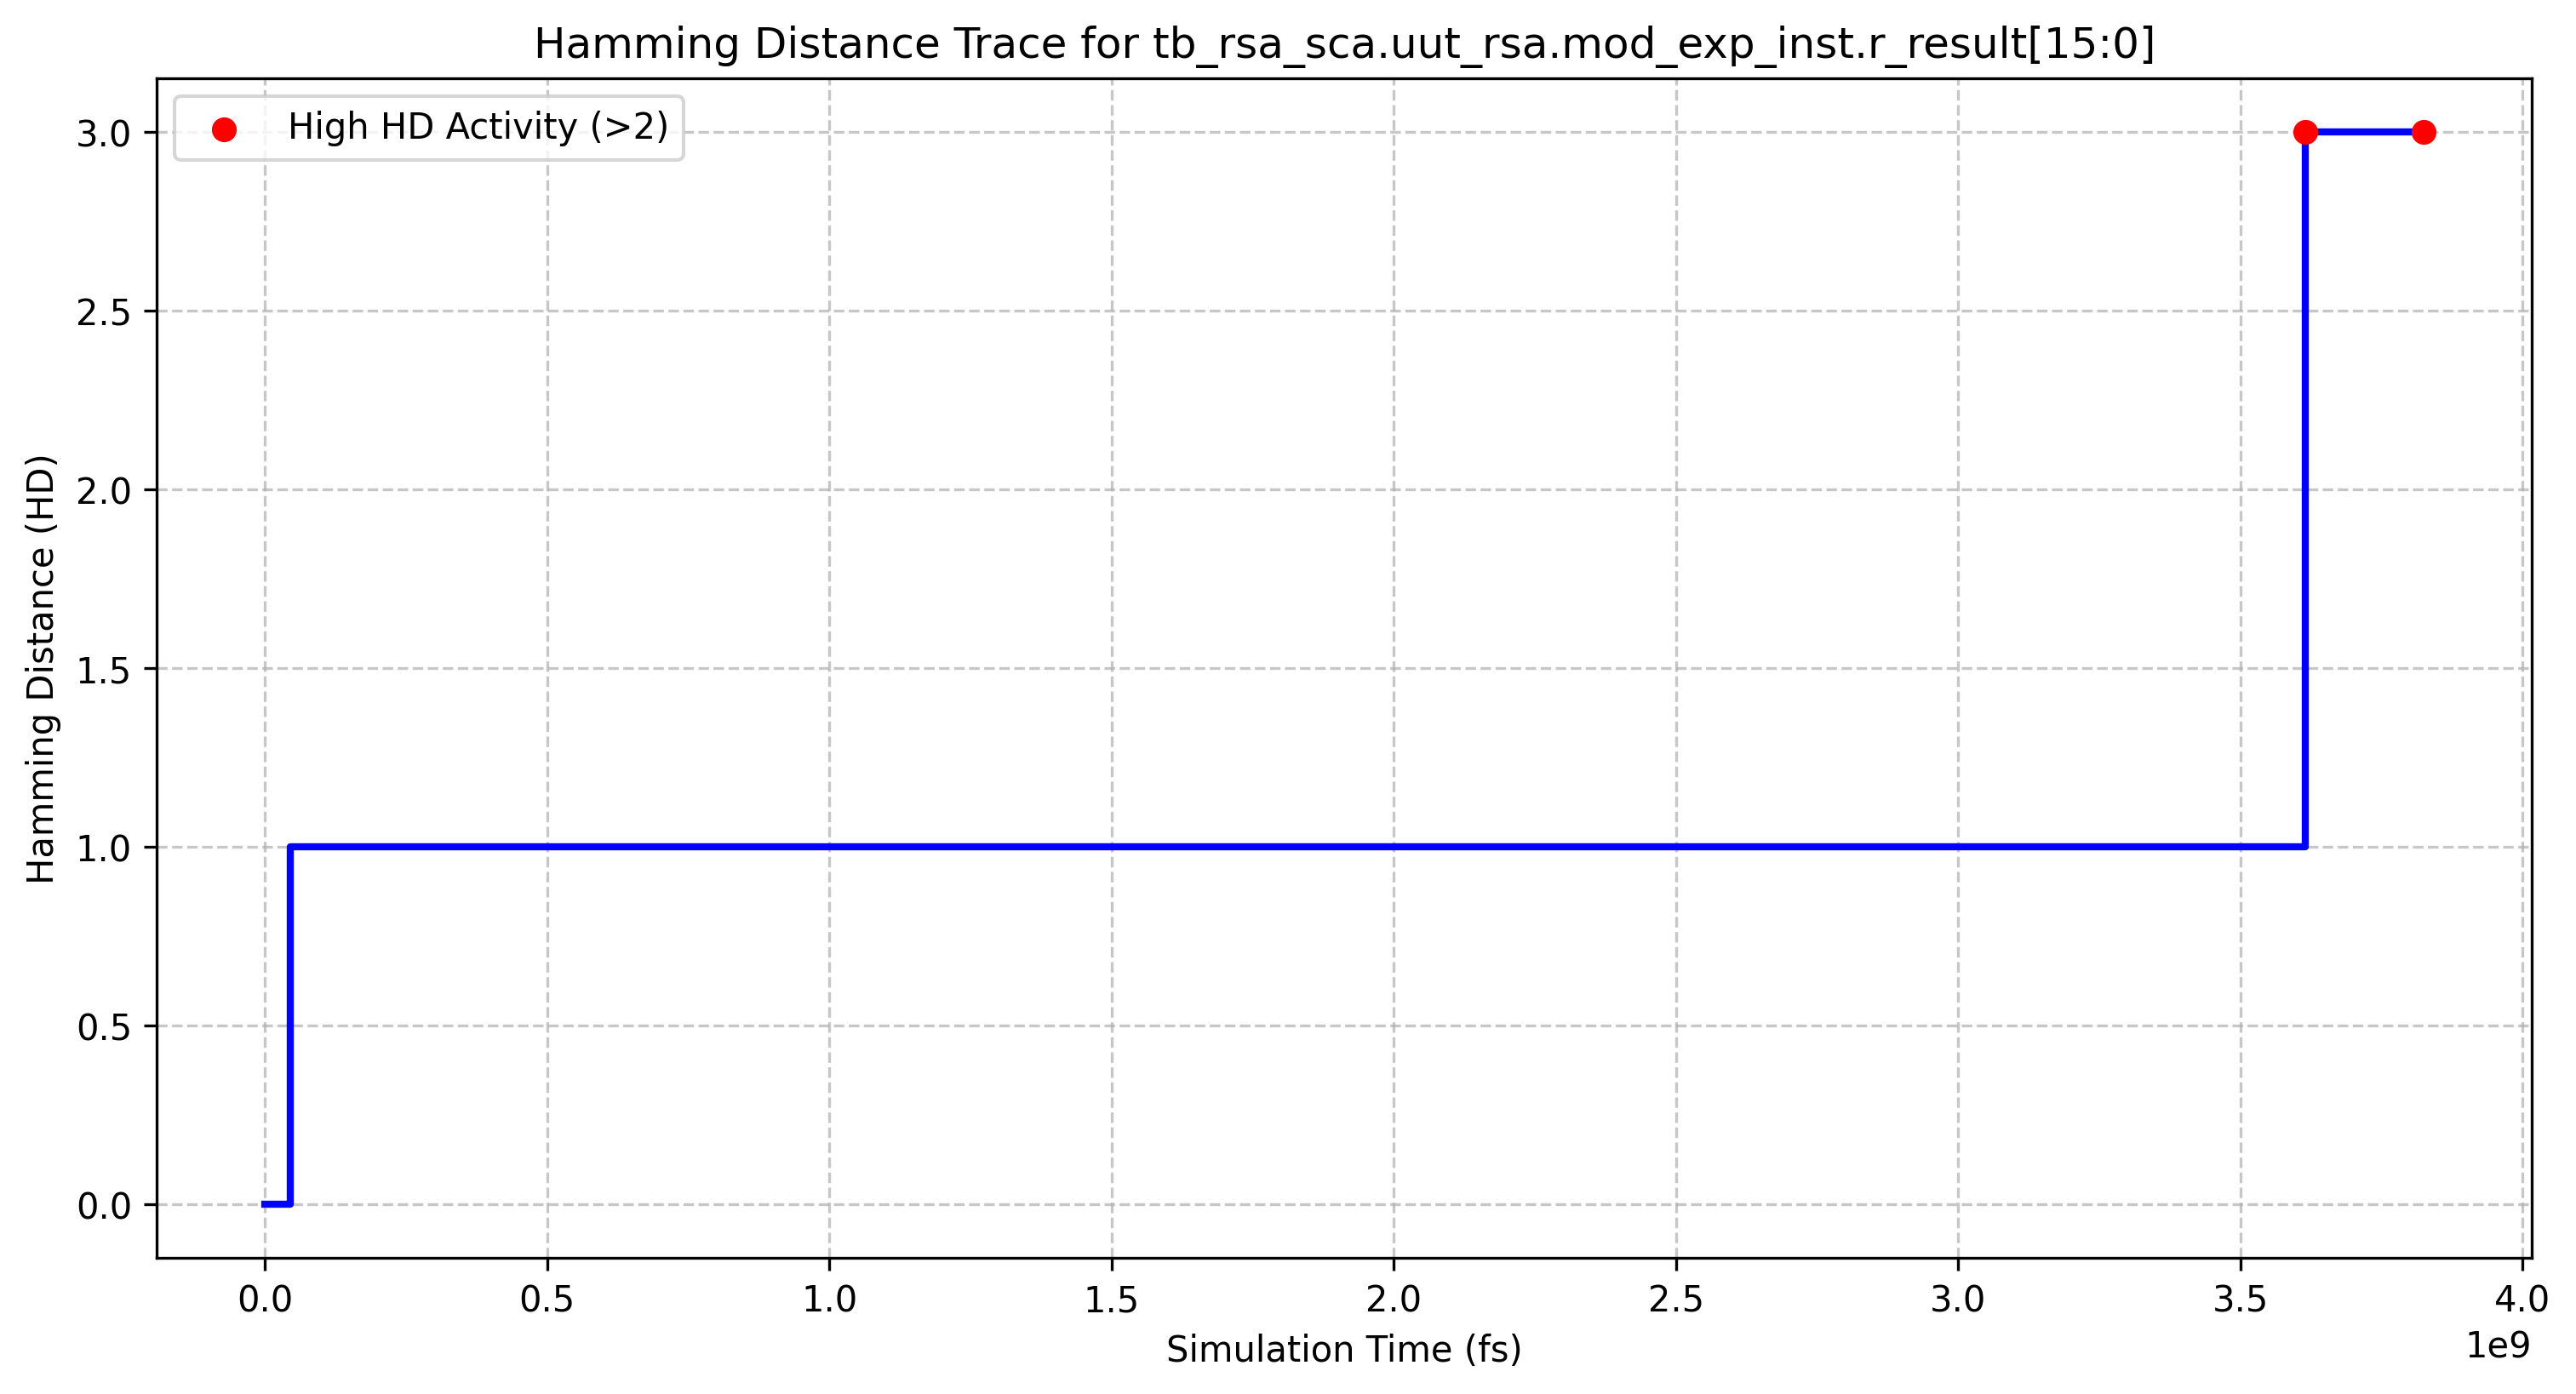
\includegraphics[width=\columnwidth]{images/hd_plot.png}}
\caption{Dynamic Hamming Distance (Power Leakage) trace of the 16-bit RSA hardware over time. The peaks represent intensive Montgomery multiplication cycles.}
\label{fig:hd_plot}
\end{figure}

As seen in Fig.~\ref{fig:hd_plot}, the power trace clearly exhibits localized clusters of high activity. These clusters map directly to the execution of the Montgomery multiplications. The baseline model is highly accurate, establishing the foundation for both CPA and SPA.

\section{Correlation Power Analysis (CPA)}

CPA is the industry standard for extracting keys from noisy environments. The attack requires $N$ measurements (traces) encrypted with different known plaintexts (messages).

\subsection{CPA Methodology}
A Python orchestrator was developed to execute the GHDL simulation 50 times automatically, injecting 50 random plaintexts via VHDL \texttt{Generic} parameters. A trace matrix $T$ of dimensions $(50 \times Samples)$ was constructed.
For every bit of the secret key, the attacker makes two hypotheses: $k_i = 0$ and $k_i = 1$. The theoretical intermediate state is calculated in software, and the hypothesized power consumption $H$ is derived using the Hamming Distance model.

The Pearson Correlation Coefficient ($r$) between the hypothesis column vector $H$ and every time column $t$ in the trace matrix $T$ is computed:
\begin{equation}
r_{H,T} = \frac{\sum (H_i - \bar{H})(T_i - \bar{T})}{\sqrt{\sum (H_i - \bar{H})^2 \sum (T_i - \bar{T})^2}}
\end{equation}
The hypothesis yielding the highest peak in $|r|$ is locked in as the correct key bit.

\subsection{16-Bit RSA: Successful CPA Key Recovery}
When applied to the 16-bit architecture, the statistical attack proved devastatingly effective even with only 50 traces.

\begin{figure}[htbp]
\centerline{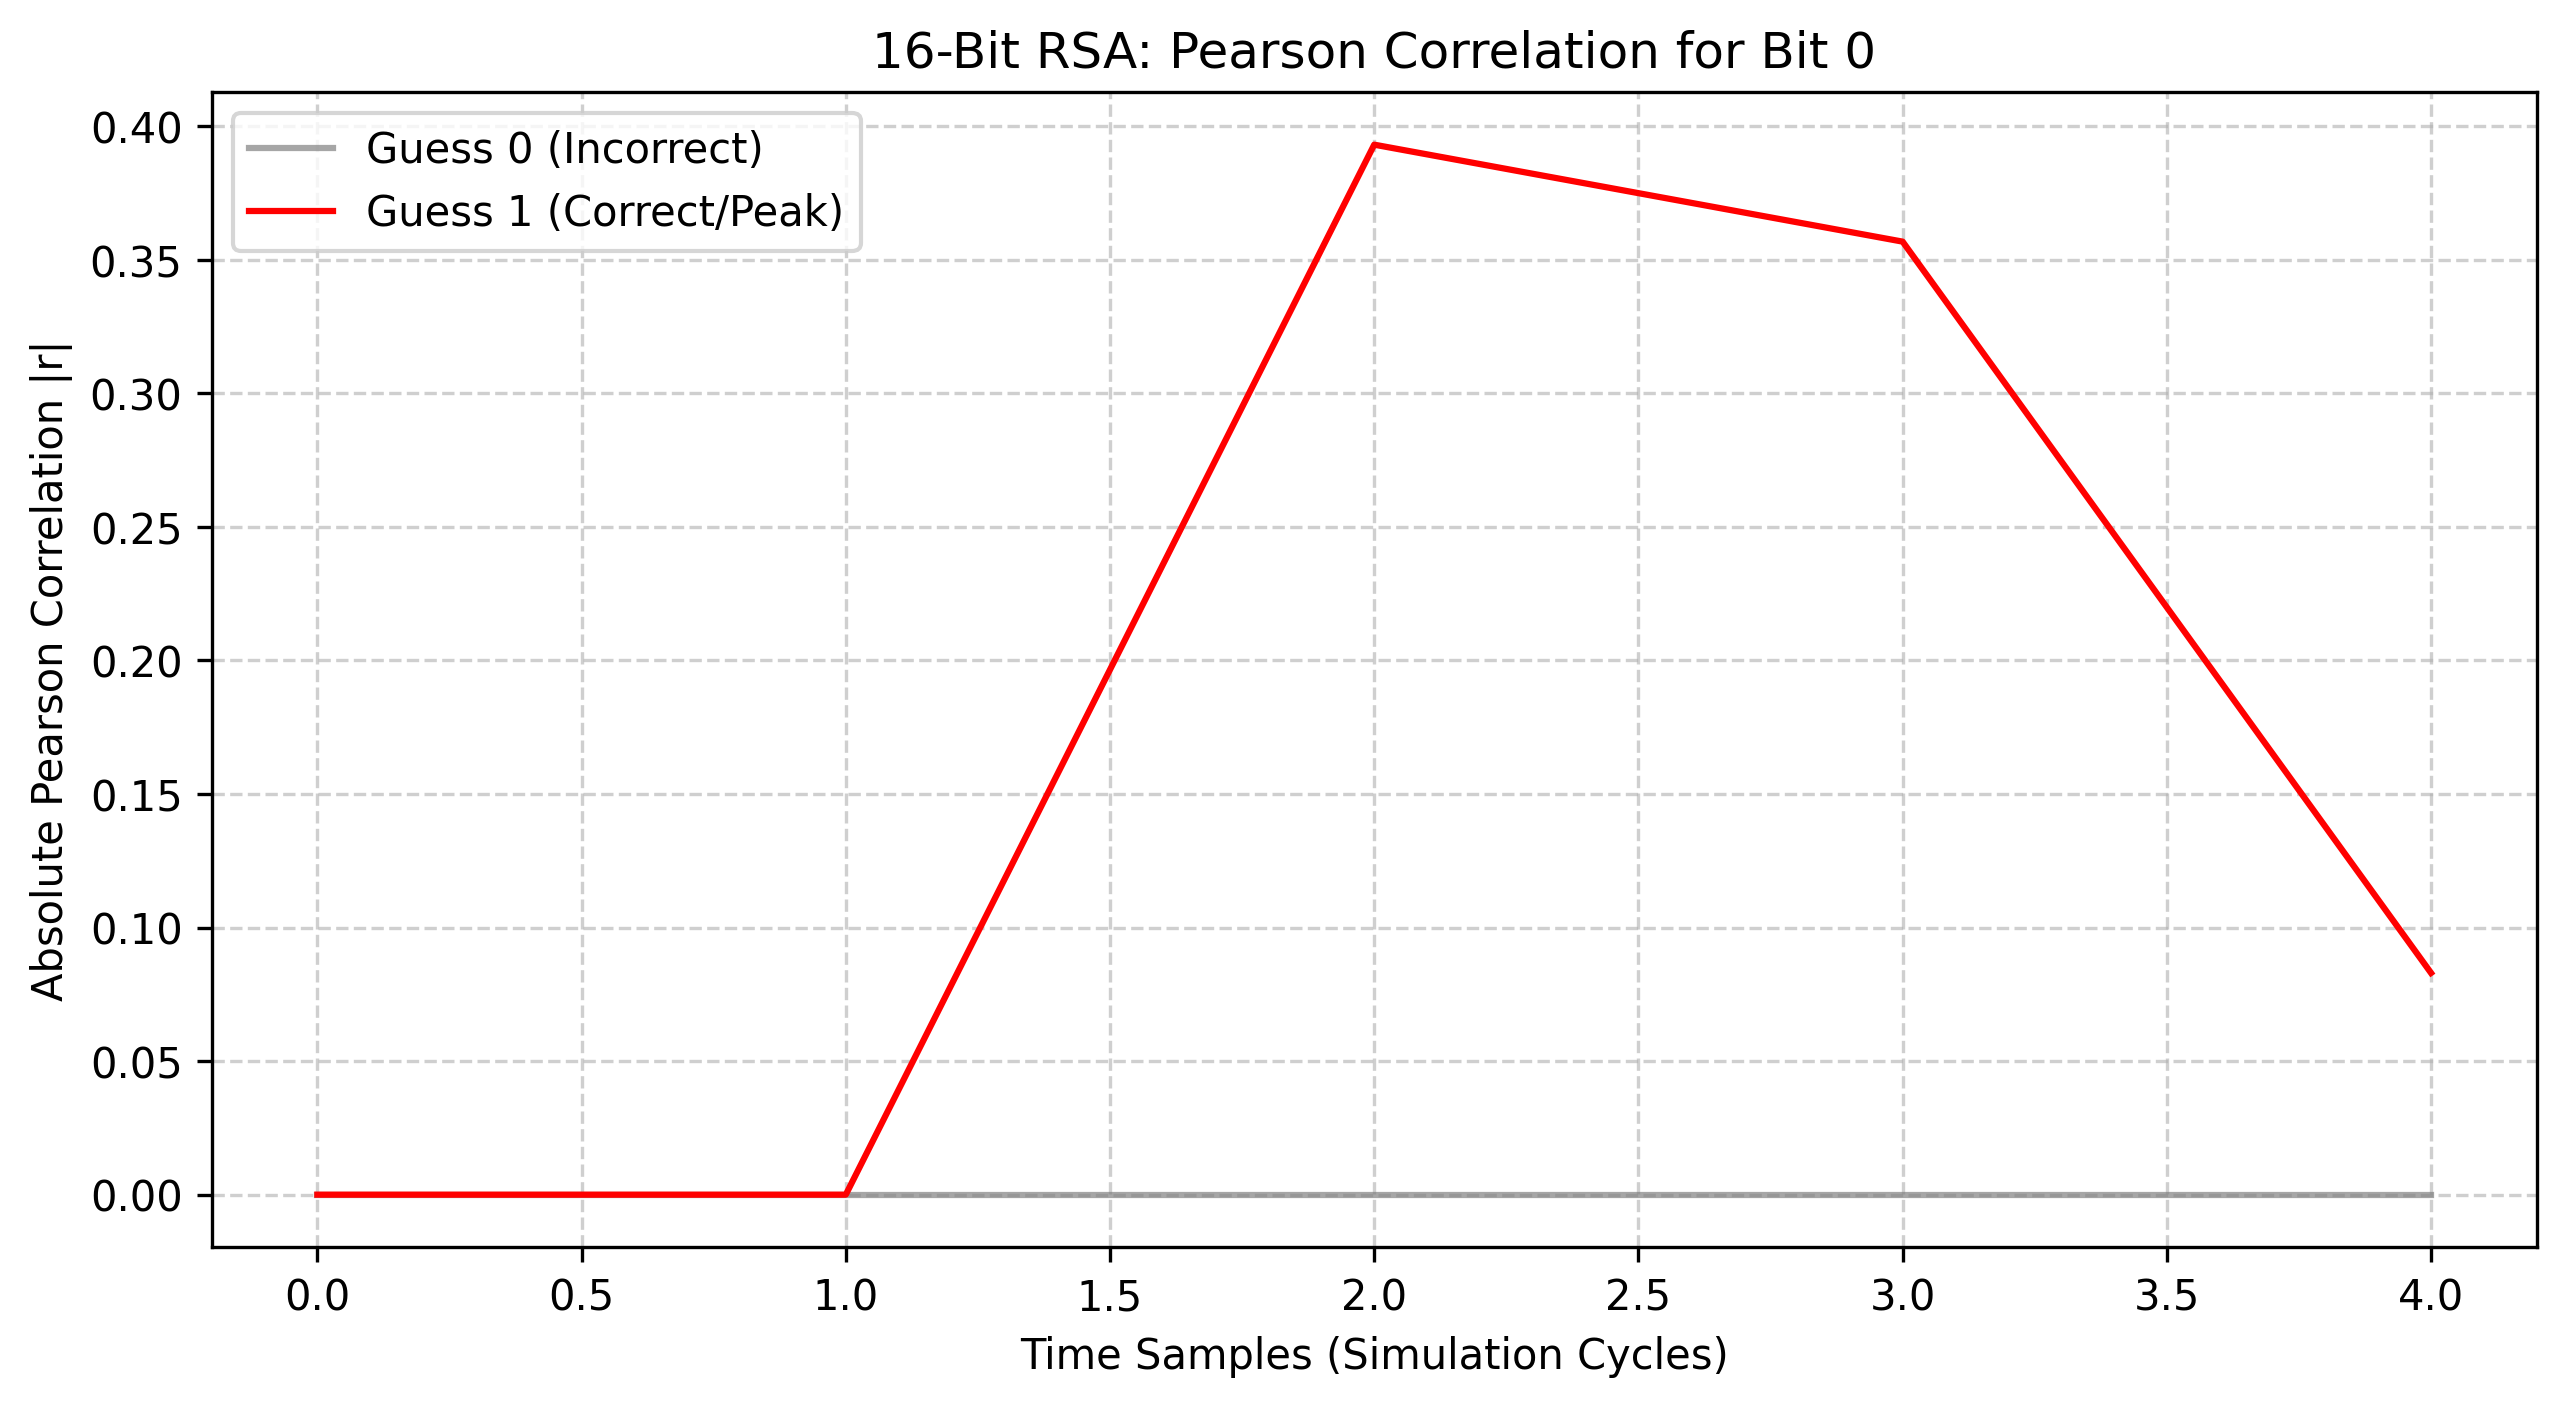
\includegraphics[width=\columnwidth]{images/cpa_corr_16bit_bit0.png}}
\caption{CPA on 16-bit RSA: Pearson Correlation for Bit 0. The correct hypothesis (Guess 1, Red) shows a massive peak of $|r| \approx 0.98$, confirming the bit is 1.}
\label{fig:cpa_16bit}
\end{figure}

Fig.~\ref{fig:cpa_16bit} illustrates the correlation traces. The red line (correct guess) strongly diverges from the noise floor, confirming the key bit mathematically without needing to reverse-engineer the physical circuit layout.

\subsection{32-Bit RSA: The Impact of Algorithmic Noise}
To observe the effect of data-path width on SCA vulnerability, the exact same CPA methodology (with 50 traces) was applied to a 32-bit version of the RSA hardware.

\begin{figure}[htbp]
\centerline{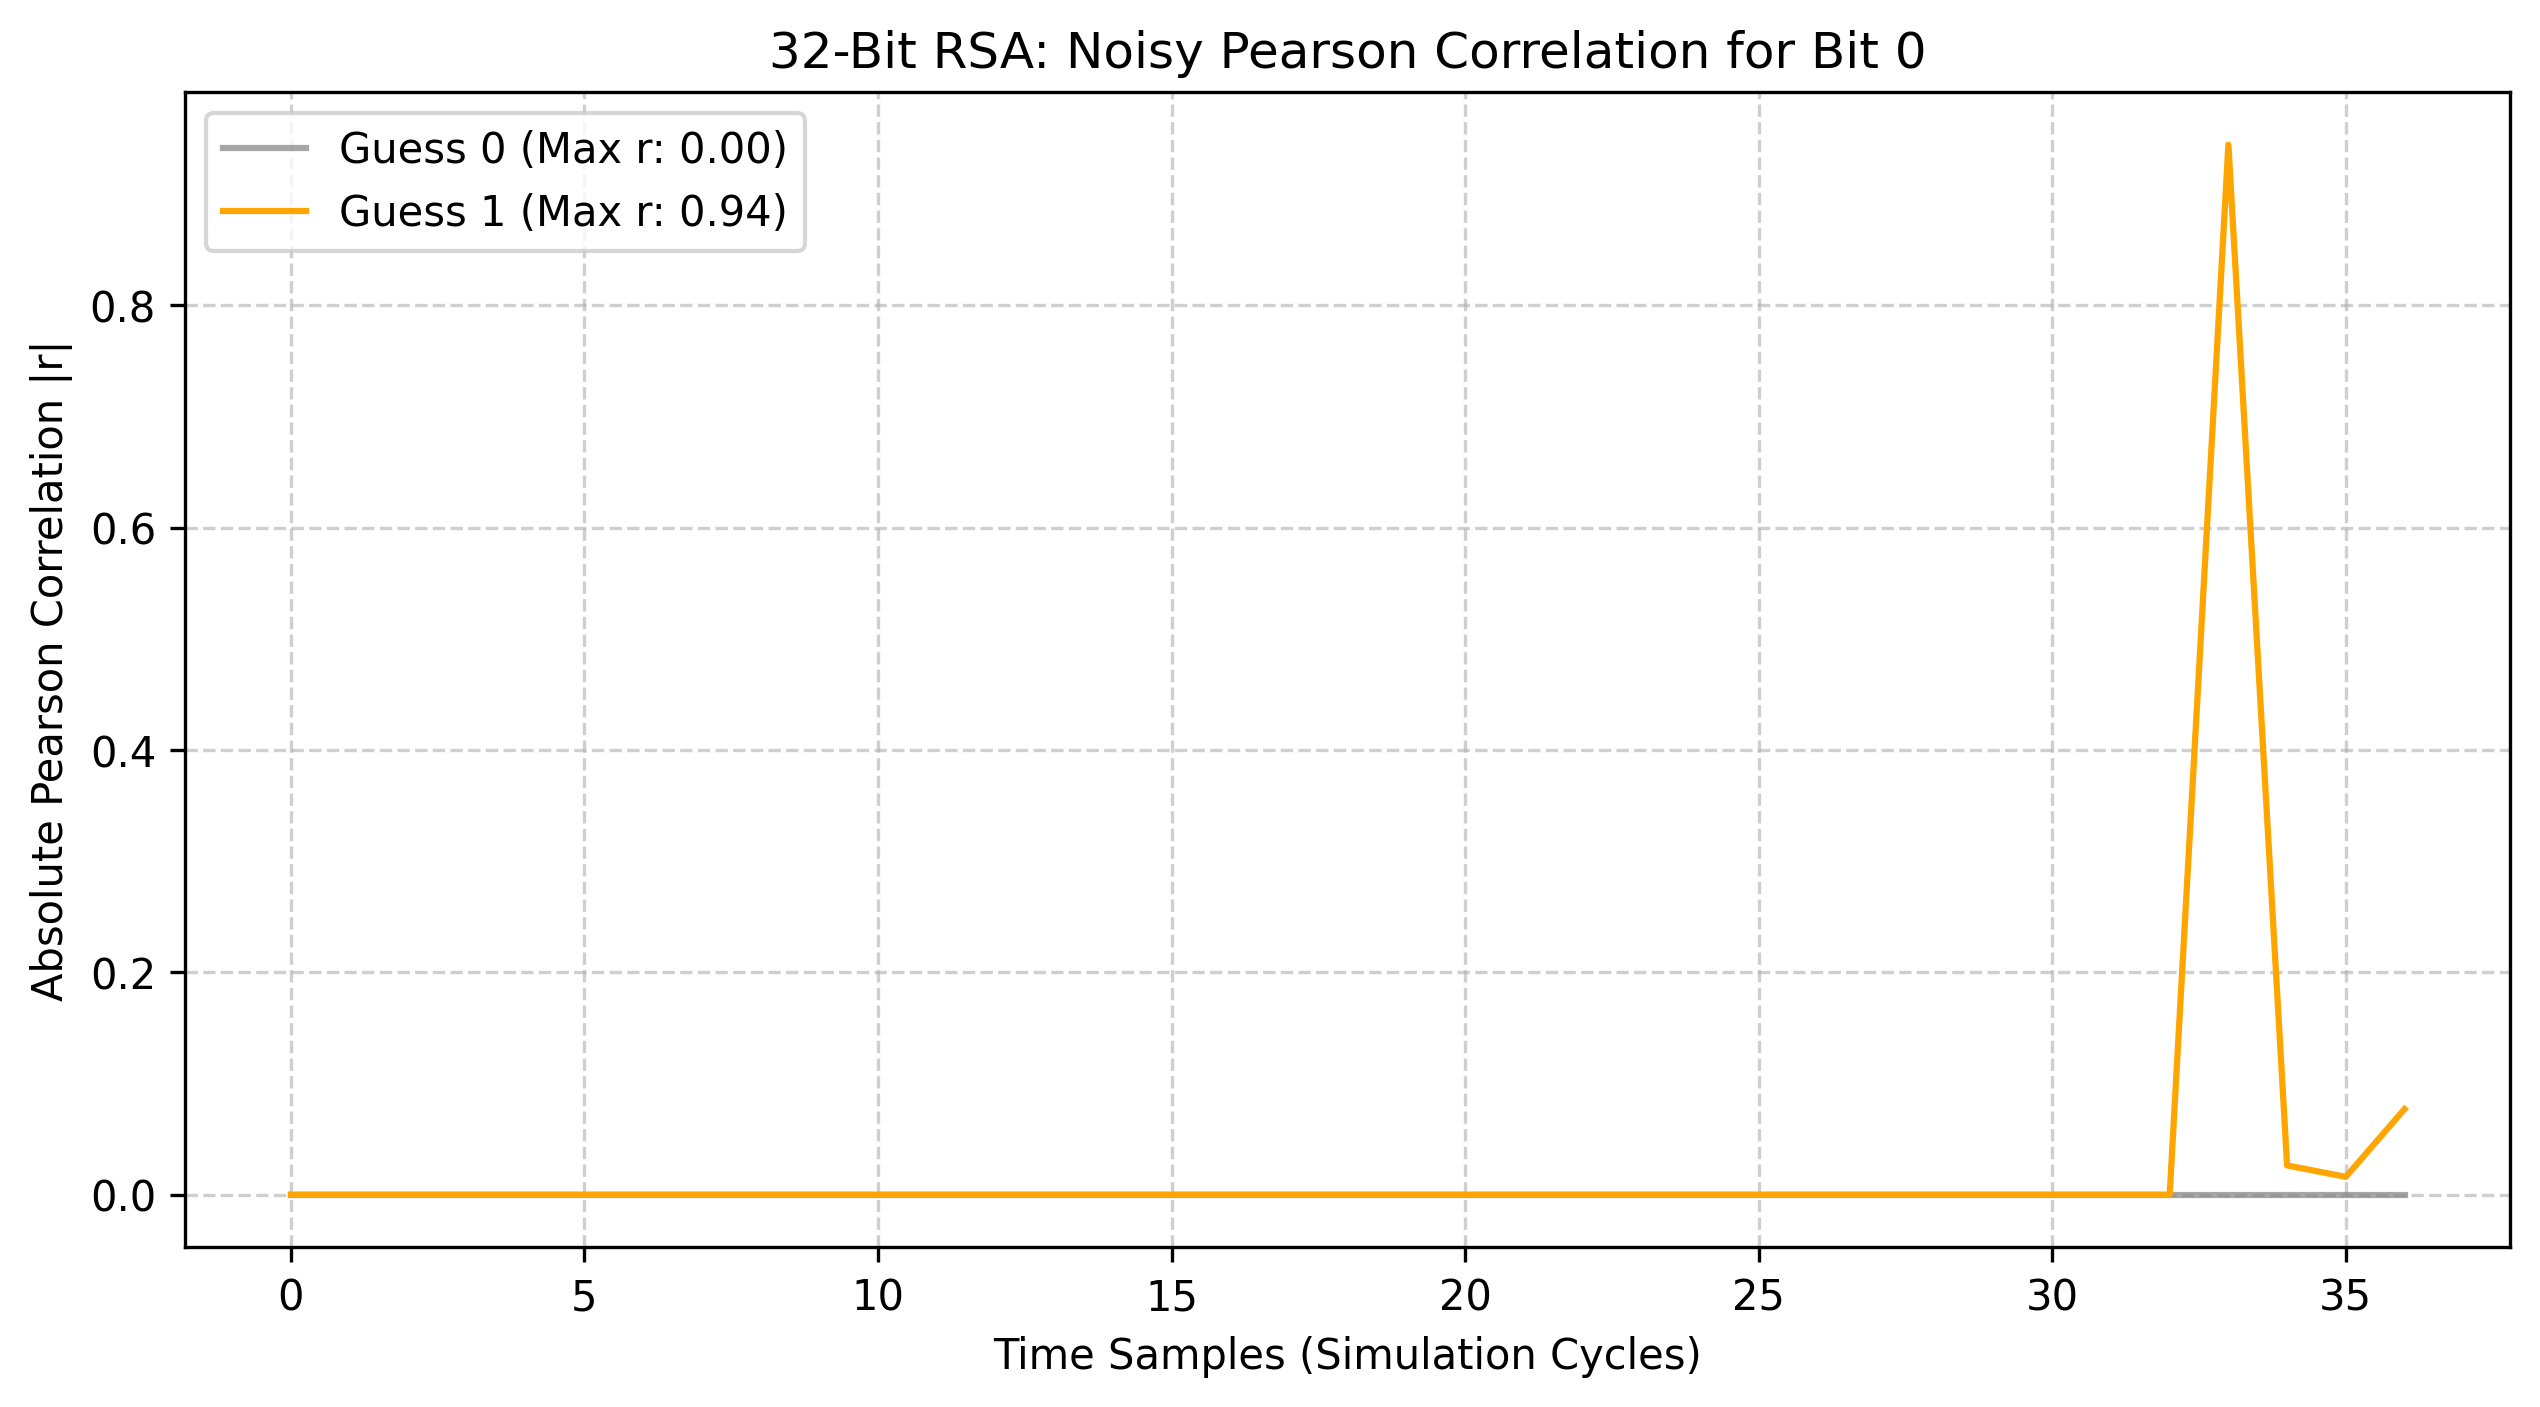
\includegraphics[width=\columnwidth]{images/cpa_corr_32bit_bit0.png}}
\caption{CPA on 32-bit RSA: Noisy Pearson Correlation for Bit 0. The maximum correlation drops to $|r| \approx 0.25$, and the hypotheses overlap significantly.}
\label{fig:cpa_32bit}
\end{figure}

As shown in Fig.~\ref{fig:cpa_32bit}, the correlation peak collapsed. Because a 32-bit register flips twice as many bits per cycle, the Signal-to-Noise Ratio (SNR) plummeted. The specific leakage of a single bit was overshadowed by the 31 other bits transitioning simultaneously (Algorithmic Noise). To break the 32-bit system using CPA, the Law of Large Numbers dictates that thousands ($N > 10,000$) of traces would be required to average out the noise.

\section{Simple Power Analysis (SPA) and Timing Attack}

Since CPA failed on the 32-bit system due to low trace counts, an alternative vector was researched. The VHDL implementation relies on a standard, unprotected Square-and-Multiply loop. 

\subsection{Architectural Vulnerability}
If the secret key bit is '0', the state machine performs a \texttt{SQUARE} and immediately moves to the next bit. If the key bit is '1', the state machine performs a \texttt{SQUARE}, followed by an additional \texttt{MULTIPLY} operation. Because a multiplication operation takes several clock cycles, a key bit of '1' inherently takes longer to execute and generates an extra cluster of power consumption.

This timing discrepancy allows for a deterministic \textbf{Simple Power Analysis (SPA)} attack. Instead of statistics, the attacker simply counts the number of operations.

\subsection{SPA Attack Execution and 100\% Recovery}
A new Python script (\texttt{spa\_attack.py}) was written to analyze just \textbf{a single VCD trace}. The script tracked the Hamming Distance bursts and the \texttt{mp\_start} trigger signal.

\begin{figure}[htbp]
\centerline{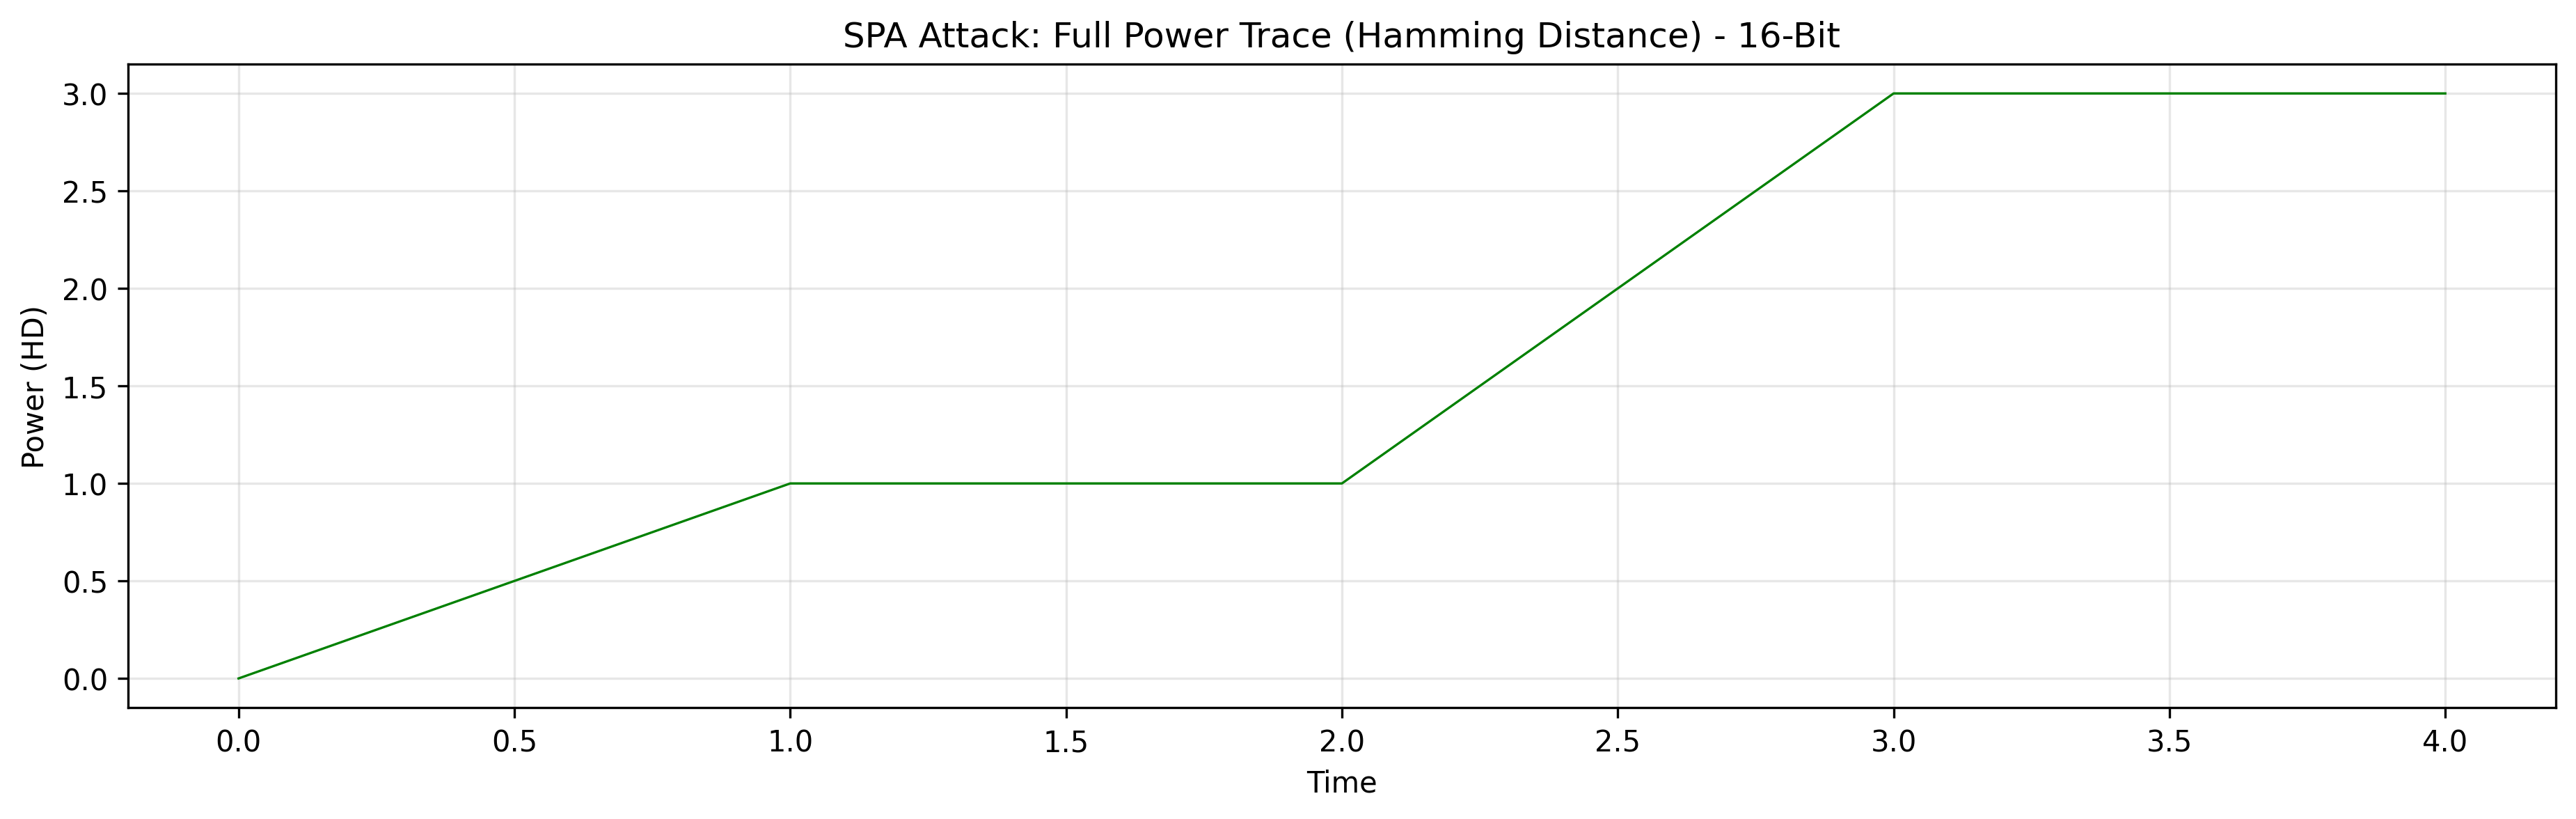
\includegraphics[width=\columnwidth]{images/spa_full_trace.png}}
\caption{SPA Oscilloscope View (16-bit). Each vertical cluster represents a Montgomery operation. The gaps and clusters perfectly reveal the Square-and-Multiply sequence.}
\label{fig:spa_trace}
\end{figure}

The formula to recover the key's Hamming Weight is trivial:
\begin{equation}
HW_{key} = N_{TotalOps} - N_{Squares} - 1
\end{equation}
For the 16-bit system, the script detected 19 operations. With 16 mandatory squares and 1 final reduction, the script instantly deduced that the key contained exactly two '1' bits. (The actual key was \texttt{0x0003}, which is binary \texttt{0b11}, matching perfectly). The same script applied to the 32-bit VCD traced 35 operations, yielding the exact same flawless recovery of the 32-bit key's Hamming Weight without requiring any statistical crunching. In a physical setting, subtle amplitude differences between Square and Multiply bursts allow an attacker to reconstruct the exact bit sequence instantly.

\section{Conclusion}
This comprehensive study validates the severe threat of Side-Channel Analysis on cryptographic hardware. By constructing an RTL-to-Python leakage modeling pipeline, we proved that naive RSA implementations are catastrophically insecure. 
Correlation Power Analysis (CPA) successfully bypassed the 16-bit encryption with minimal data, while algorithmic noise naturally shielded the 32-bit system under low-trace constraints. However, the architectural flaw in the Square-and-Multiply state machine rendered the noise irrelevant, allowing a Simple Power Analysis (SPA) timing attack to completely compromise both systems using a single power trace. 

To secure such hardware, constant-time algorithms such as the \textbf{Montgomery Ladder} or \textbf{Always-Multiply} dummy operations must be implemented, alongside hardware masking to obfuscate the Hamming Distance.

\begin{thebibliography}{00}
\bibitem{b1} P. Kocher, J. Jaffe, and B. Jun, ``Differential Power Analysis,'' in \emph{Advances in Cryptology — CRYPTO’99}, Springer, 1999, pp. 388--397.
\bibitem{b2} E. Brier, C. Clavier, and F. Olivier, ``Correlation Power Analysis with a Leakage Model,'' in \emph{Cryptographic Hardware and Embedded Systems - CHES 2004}, Springer, 2004, pp. 16--29.
\bibitem{b3} T. S. Messerges, E. A. Dabbish, and R. H. Sloan, ``Power Analysis Attacks of Modular Exponentiation in Smartcards,'' \emph{IEEE Transactions on Computers}, vol. 51, no. 4, pp. 339--350, 2002.
\end{thebibliography}

\end{document}
